\section{Parallelization Techniques}
\label{sec:parallel}

Here we survey three powerful techniques behind a recent trend of work on
constant-depth circuits. The first is the constant-depth unbounded fan-out.
The second is the parallelization of
commuting gates and the \textsc{OR} reduction of H{\o}yer and {\v S}palek
\cite{Hoyer2002}. This reduction gives us an approximate \textsc{OR} gate,
which is made exact by Takahashi and Tani \cite{Takahashi2011} using the
third technique, the analysis of boolean parity functions.

%%%%%%%%%%%%%%%%%%%%%%%%%%%%%%%%%%%%%%%%%%%%%%%%%%%%%%%%%%%%%%%%%%%%%%%%%%%%%%
\subsection{Unbounded Fanout}

In classical
circuits, the ability to copy bits is taken for granted. However,
in quantum circuits,
it is impossible to create an unentangled copy of a general quantum state, a
principle known as ``no-cloning'' \cite{Nielsen2000}. However,
it \emph{is} possible to create entangled copies by transversally applying
the CNOT gate to corresponding qubits in the source and destination register.
One can copy one source qubit $\ket{\psi} = \alpha \ket{0} + \beta \ket{1}$
to $n$ target qubits in this manner according to Equation \ref{eqn:copy}.

\begin{equation}
(\alpha \ket{0} + \beta \ket{1}) \otimes \ket{0}^{\otimes n} \rightarrow
\alpha \ket{0}^{\otimes (n+1)} + \beta \ket{1}^{\otimes (n+1)}
\label{eqn:copy}
\end{equation}

This can be done in logarithic depth with a cascade of CNOTs as shown
in Figure \ref{fig:fanout}.

\begin{figure}
\begin{center}
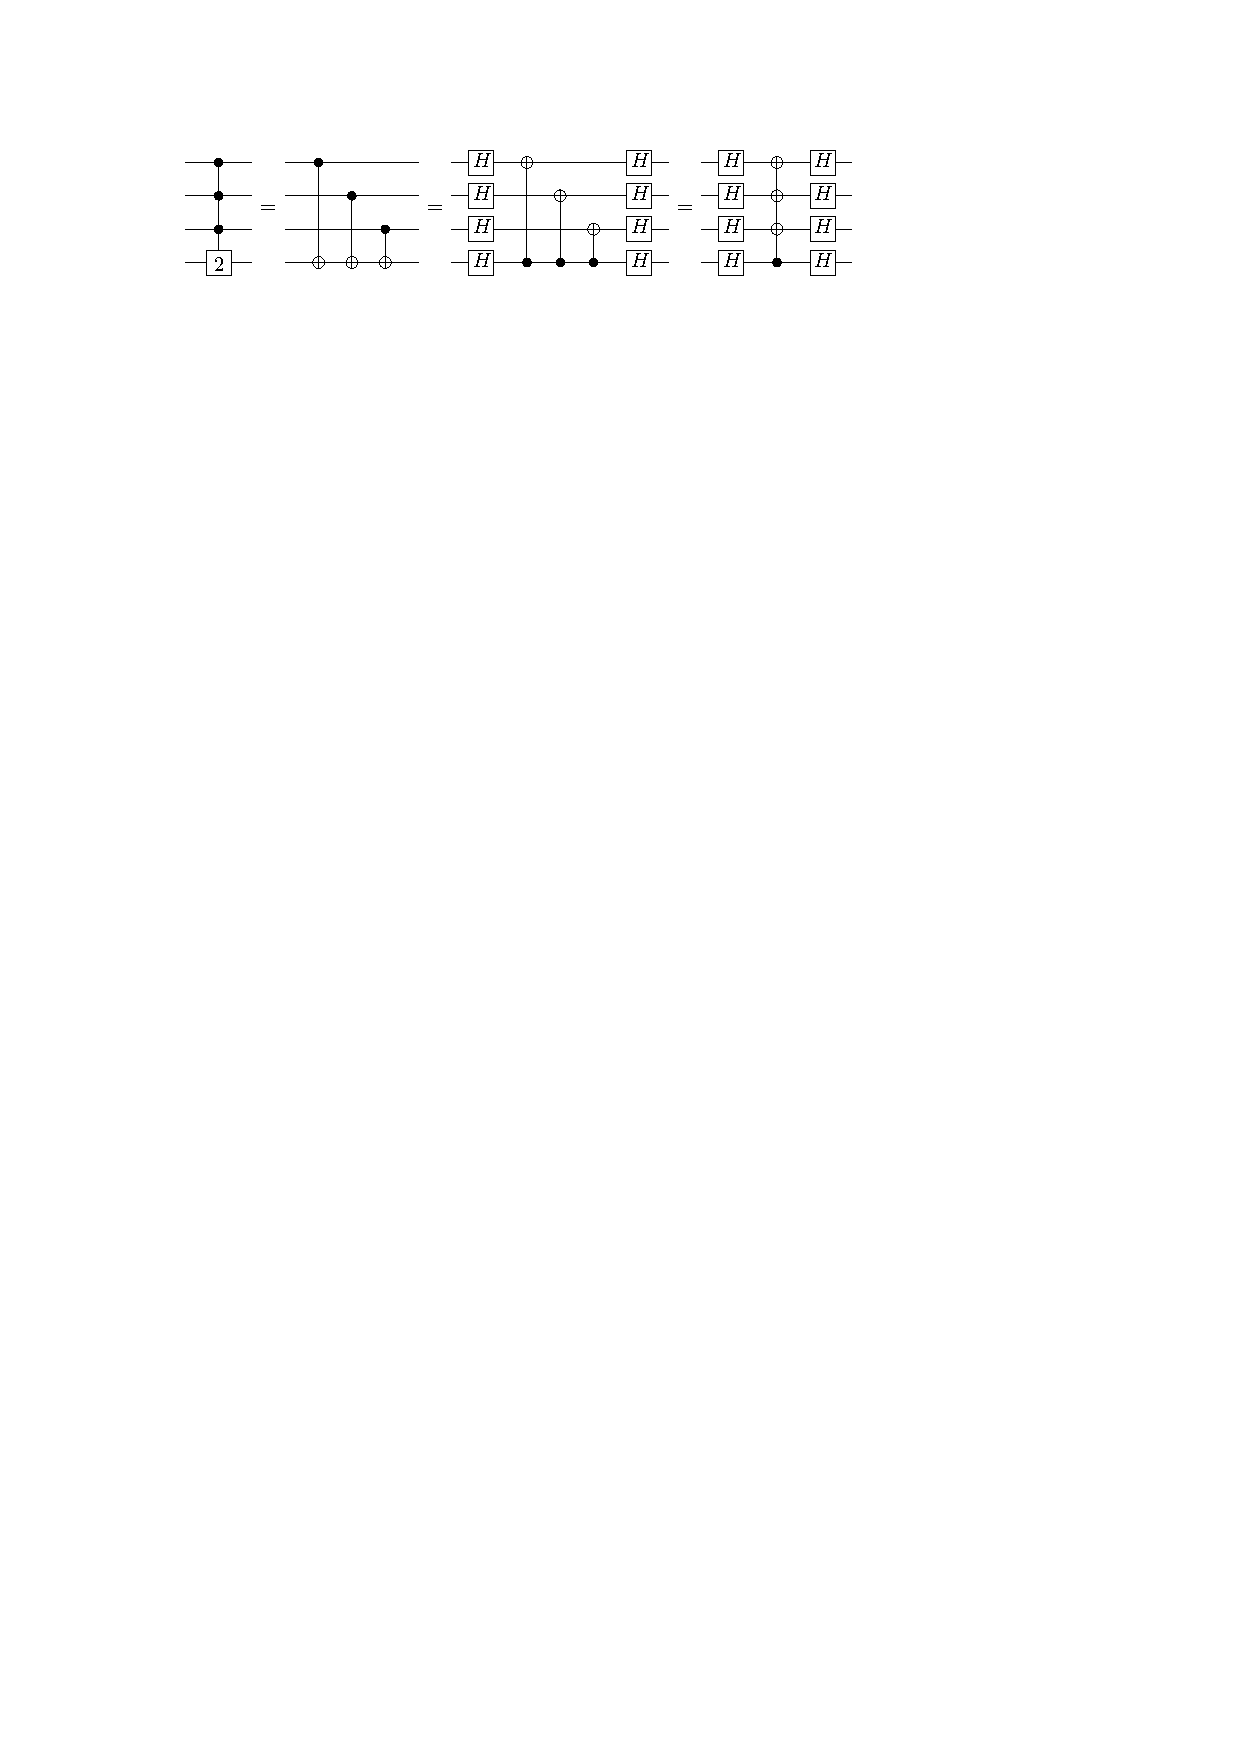
\includegraphics[width=3in]{figures/fanout.pdf}
\caption{The equivalence of unbounded fan-out and parity gates on 3 qubits \cite{Hoyer2002}.}
\label{fig:fanout}
\end{center}
\end{figure}

Moore and Nilsson showed unbounded fan-out was equivalent in power to the parity gate
\cite{Moore1998}, also via the example shown in Figure \ref{fig:fanout}.
H{\o}yer and {\v S}palek have studied it in the
context of constant-depth circuits over a fixed basis ($\textsc{QNC}_f^0$)
to approximate a wide variety of unbounded logic gates \cite{Hoyer2002} which
we will discuss in the next section.

This has also been used in adder circuits by Takahashi and Tani
\cite{Takahashi2009} to achieve $O(\log^* n)$ depth.
These gates are not just of theoretical interest; some physical systems
such as ion traps admit the implementation of efficient multi-qubit gates,
following the work of M{\o}lmer and S{\o}rensen \cite{Sorensen1999}.
Recently unbounded fanout gates have also been implemented in 2D architectures using
constant-depth cat-state creation in $n$ ancillary qubits to
implement $n$-qubit controlled operations \cite{Rosenbaum2012} and
factoring in polylogarithmic-depth on a \textsc{2D NTC} architecture
\cite{Pham2012b}.
An $n$-qubit cat state is shown in Equation \ref{eqn:cat}; it is the
maximally entangled $n$-qubit state which is an equal superposition of all
$\ket{0}$'s and all $\ket{1}$'s.
However, unbounded fanout consumes the cat state,
in that it is not possible to uncompute the cat state after its use. This is
a severe caveat in its use in physical implementations.

\begin{equation}
\label{eqn:cat}
\ket{\Phi_n} = \frac{1}{\sqrt{2}}
\left(\ket{0}^{\otimes n} + \ket{1}^{\otimes n}\right)
\end{equation}

%%%%%%%%%%%%%%%%%%%%%%%%%%%%%%%%%%%%%%%%%%%%%%%%%%%%%%%%%%%%%%%%%%%%%%%%%%%%%%
\subsection{Commuting Operator Parallelism and Approximate \textsc{OR}}

Gates applied to different qubits can be applied at the same time. This is
the classical definition of parallelism. However, there is an inherently
quantum form of parallelism described by H{\o}yer and {\v S}palek
\cite{Hoyer2002}. Any two commuting operations
can be performed as the same time, provided that (1) we have access to
unbounded fan-out and (2) that we can efficiently transform
into the basis where they are both diagonal.
This second condition is the case for many
functions needed in quantum algorithms, for example modular arithmetic
\cite{Moore1998}, and the constant-depth rotation by Hamming weight shown
in Figure \ref{fig:rotate-hamming}. This is the underlying technique to
the approximate \textsc{OR} circuit that we will now expose.

\begin{figure}
\begin{center}
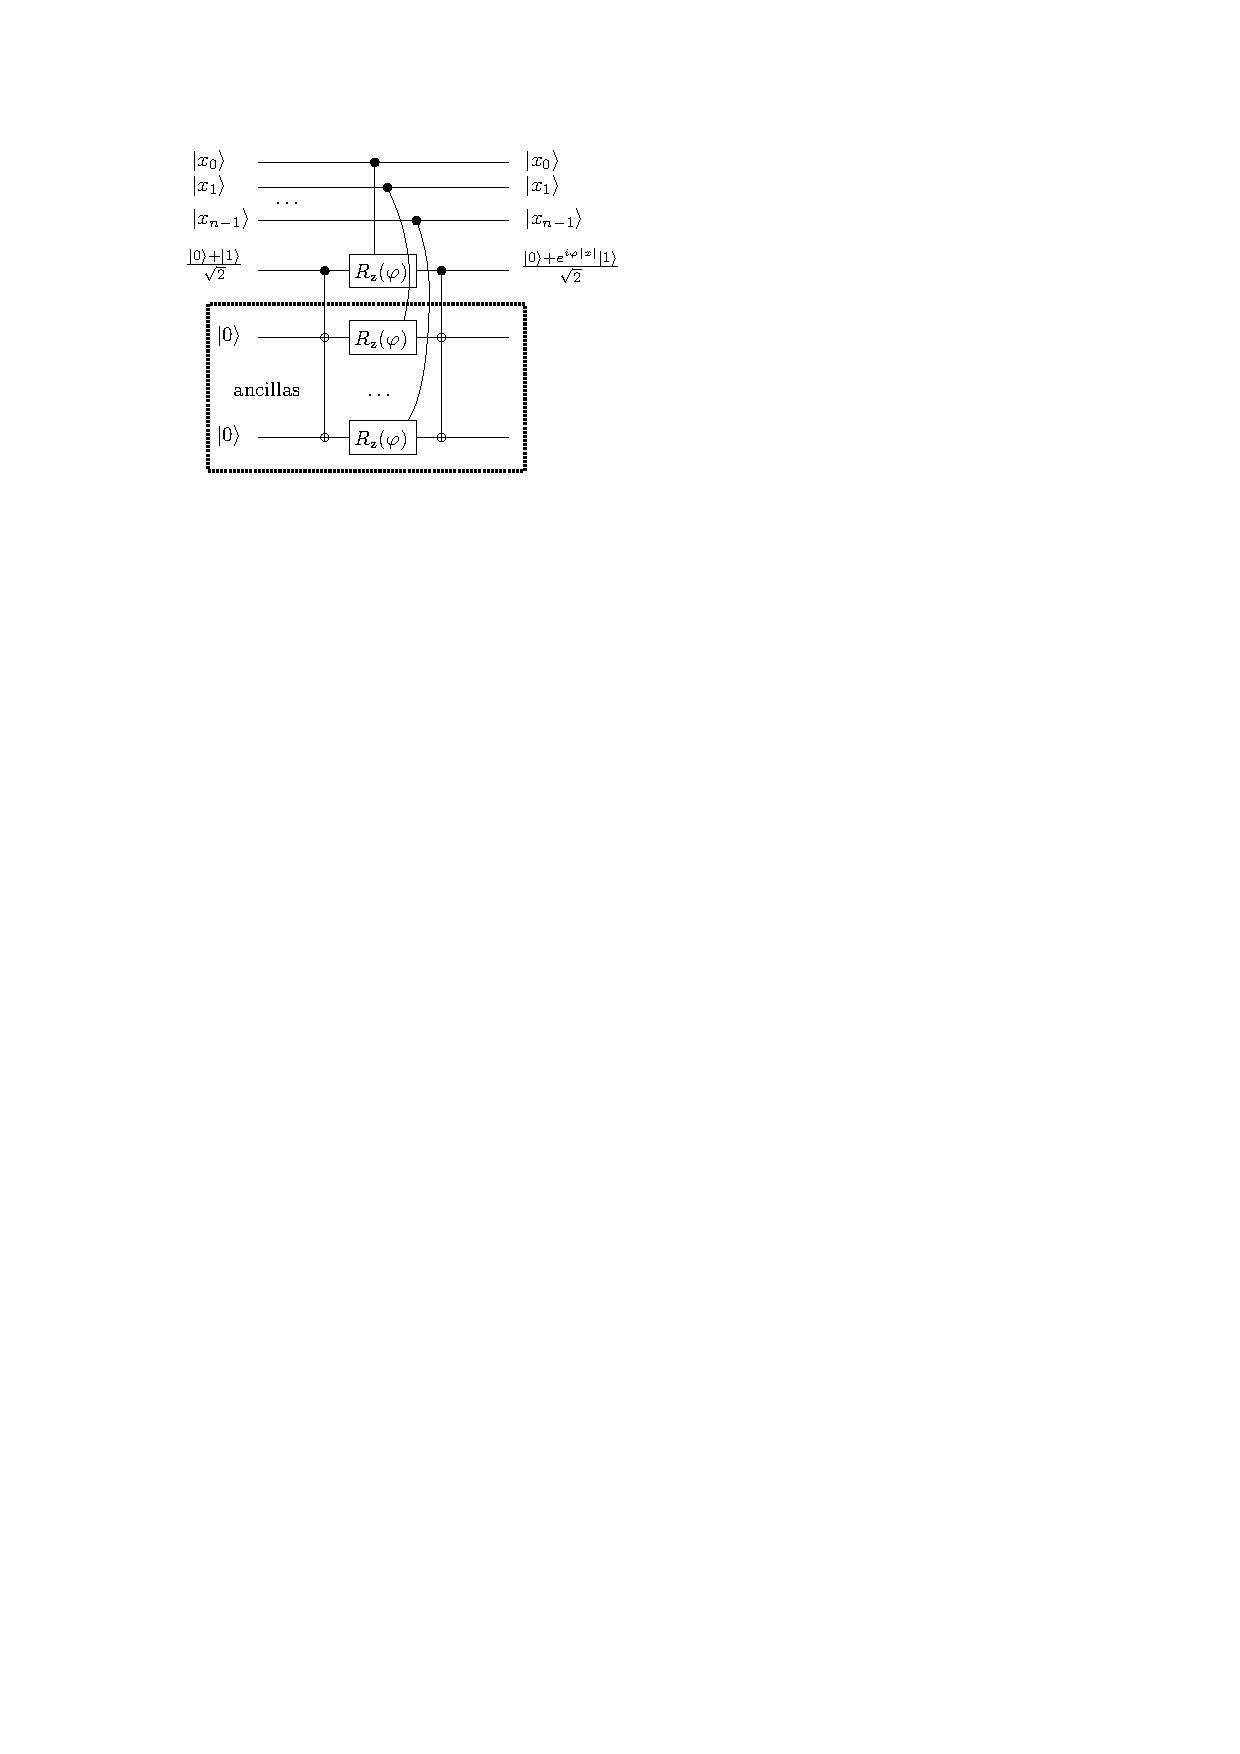
\includegraphics[width=2.5in]{figures/rotate-hamming.pdf}
\caption{Constant-depth rotation by Hamming weight $|x|$ \cite{Hoyer2002}.}
\label{fig:rotate-hamming}
\end{center}
\end{figure}

We can define the \textsc{OR} function on an $n$-bit string $x$ in terms of
its Hamming weight
$|x|$. Note that \textsc{OR} is a classical function, but that we are using quantum
techniques to approximate it.

\begin{equation}
\textsc{OR}(x) =
\begin{cases}
0 & \text{if } |x| = 0\\
1 & \text{if } |x| \ne 0
\end{cases}
\end{equation}

Using the circuit in Figure \ref{fig:rotate-hamming}, which computes the
rotation $R_Z(\phi|x|)$ for any angle $\phi$,
one can see how to distinguish $|x|=0$ from
$|x| \approx \frac{n}{2}$ (by setting $\phi=2\pi$).
We need an extra trick to ``mix up'' the
rotation for \emph{any} $|x| \ne 0$ so that its measurement statistics are fairly
close to the $|x| = \frac{n}{2}$ case.

Define the following notation in Equation \ref{eqn:mu-rotate2}
for a single-qubit ancilla state $\ket{\mu^{|x|}_{\phi_k}}$ that
encodes rotation by Hamming weight times a multiple $\phi_k = \frac{2\pi}{m}k$,
where we define $m$ later.
The efficient
preparation of this state is shown in Equation \ref{eqn:mu-rotate1}.

\begin{eqnarray}
\label{eqn:mu-rotate1}
\ket{\mu^{|x|}_{\phi_k}} & = & (H \cdot R_z(\phi_k|x|) \cdot H) \ket{0} \\
                         & = &
\label{eqn:mu-rotate2}
\frac{1 + e^{i\phi_k|x|}}{2}\ket{0} + \frac{1 - e^{i\phi_k|x|}}{2}\ket{1}
\end{eqnarray}

Then we fan out the $n$ bits of our input, $\{\ket{x_1}, \ldots, \ket{x_n}\}$,
$m$ times each into ancillae, and compute $m$ values of
$\ket{y_k} = \ket{\mu^{|x|}_{\phi_k}}$ for each $n$-qubit block of ancillae.
The expected Hamming weight of this new $m$-bit register $\ket{y}$, formed by
the result bits $\ket{y_k}$, is now shown in Equation \ref{eqn:expected-y}.
Here we make use of the Hoeffding Lemma \cite{Hoeffding1963},
which requires that we set
$m = n \log n$.

\begin{equation}
\label{eqn:expected-y}
E[|Y|] =
\begin{cases}
0 & \text{if } |x| = 0\\
\frac{m}{2} & \text{if } |x| \ne 0
\end{cases}
\end{equation}

This is the reduction that we wanted in the beginning of this section, and
we now recursively feed $\ket{y}$ into a circuit for $R_Z(2\pi|y|)$ to get
the final result bit $\ket{z} = \ket{\mu_{\phi_1}^{|y|}}$, which is
the approximate \textsc{OR} of the original input $x$.
The entire circuit shown in Figure \ref{fig:or-approx}.

\begin{center}
\begin{figure}
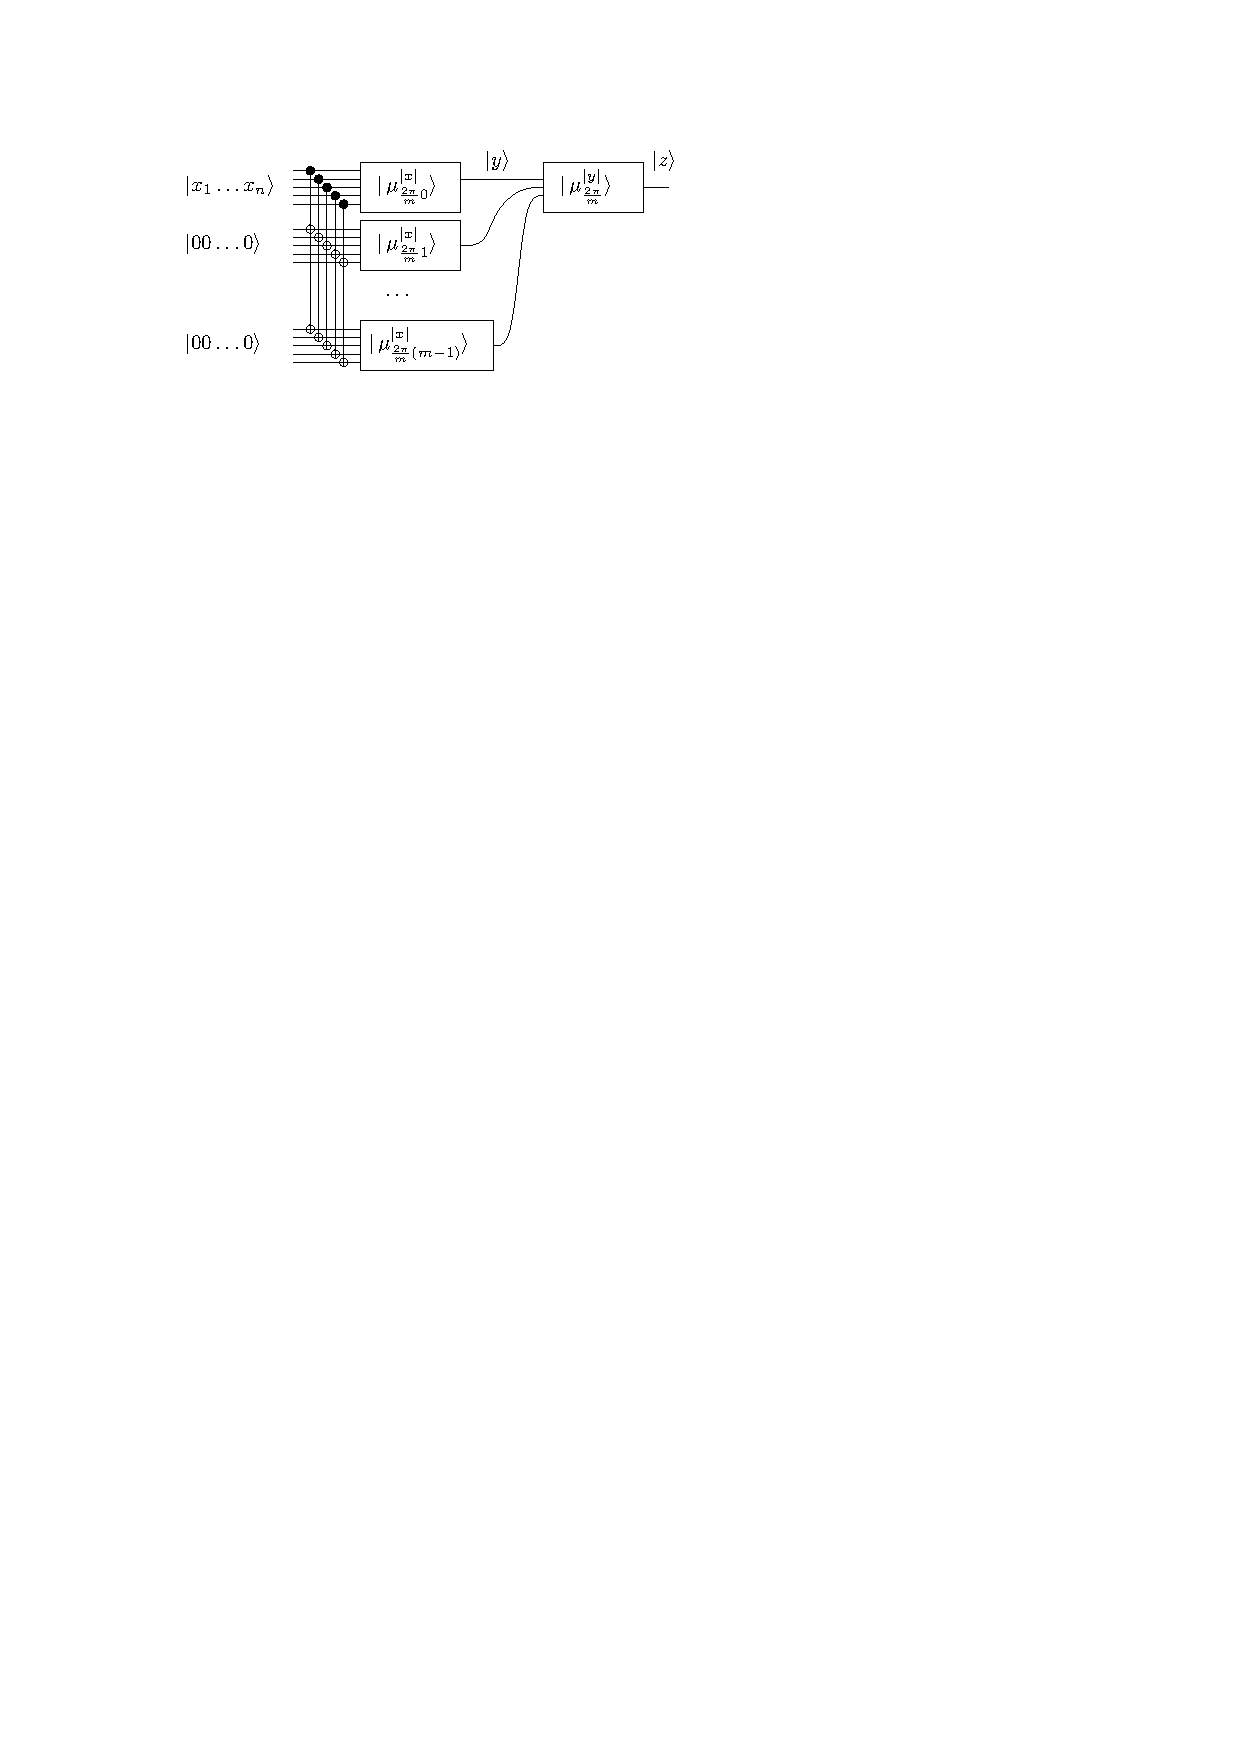
\includegraphics[width=3in]{figures/or-approx.pdf}
\caption{\textsc{OR} approximation by parallel Hamming weight rotations \cite{Hoyer2002}.}
\label{fig:or-approx}
\end{figure}
\end{center}

This circuit has one-sided error $\epsilon = \frac{1}{n}$ in depth $O(1)$,
size $O(n^2 \log n)$, and width $O(n^2 \log n)$.
%Its space is just the product of the width and depth, $O(n^2 \log n)$.

As an interesting corollary,
H{\o}yer and {\v S}palek also discovered an exact reduction to go from an \textsc{OR} gate
on $n$ bits to an \textsc{OR} gate on $m=\lceil \log(n+1) \rceil$ bits, also in
constant depth and with both size and width increasing as $O(n \log n)$.
They use this \emph{\textsc{OR} reduction} to get constant-depth
circuits for approximating the QFT, the exact gate $\textsc{EX}[t]$, the counting gate CO,
the threshold gate $\textsc{TH}[t]$, and the majority gate $\textsc{MAJ}$.
By recursively applying this reduction and related techniques, they
get an $O\log^*{n}$ depth circuit for approximate \textsc{OR},
where $\log^*n$ is the iterated logarithm function and is essentially constant
($c < 6$ given the number of particles in the universe).

%The essential concept between the \textsc{OR} reduction is to reduce computing the
%	extsc{OR} of $n$ qubits to computing the 	extsc{OR} of $\log n$ qubits in constant depth.
%Once this has been done, one can apply the reduction recursively to reduce
%the 	extsc{OR} of $\log n$ qubits to the 	extsc{OR} of $\log \log n$ qubits, until we
%are left with a constant number of qubits that we can take the 	extsc{OR} of
%in the obvious way.

%%%%%%%%%%%%%%%%%%%%%%%%%%%%%%%%%%%%%%%%%%%%%%%%%%%%%%%%%%%%%%%%%%%%%%%%%%%%%%
\subsection{Parity Function Decomposition and Exact \textsc{OR}}

However, what cares the true theorist about the number of particles in the
universe? This leaves
a gaping open question whether we can get an \emph{exact} \textsc{OR} circuit in truly
constant depth. Takahashi and Tani answered this question in the
affirmative \cite{Takahashi2011}.
This also resolves the relative statuses of
three constant-depth circuit complexity classes. $\textsf{QNC}^0_f$ is the
class of constant-depth circuits over single-qubit gates and CNOT.
$\textsf{QAC}^0_f$ augments this set with an unbounded \textsc{OR} gate.
$\textsf{QTC}^0_f$ augments this further with a threshold gate.

\begin{equation}
\label{eqn:qcc}
\textsf{QNC}_f^0 = \textsf{QAC}_f^0 = \textsf{QTC}_f^0
\end{equation}

Equation \ref{eqn:qcc} is surprising because there is a separation between
the classical equivalents.
Namely, $\textsf{NC}^0_f \subsetneq \textsf{AC}^0_f \subseteq \textsf{TC}^0_f$,
and this gives us a further clue about the potential power of quantum
versus classical computing.

The exact \textsc{OR} circuit consists of two stages. The first stage is the
\textsc{OR}
reduction of H{\o}yer and {\v S}palek from $n$ bits to $O(\log n)$ bits
described in the previous section.
The second stage is an exact \textsc{OR} circuit which 
decomposes of \textsc{OR} into masked parity functions,
similar to the Fourier analysis of Boolean functions \cite{ODonnell2008},
which we show in Equation \ref{eqn:pa-decomp}.
The exact \textsc{OR} circuit takes as input $m$ bits and operates in
$O(1)$ depth and with
size and width both in $O(m\cdot2^m)$. This last figure is exponential in $m$,
which is why it is necessary to perform the reduction in the first stage,
so that $m = O(\log n)$, and $O(\log n \cdot 2^{\log n}) = O(n \log n)$ still
gives us polynomial size and width.

\begin{equation}
\textsc{OR}_n(x) = \frac{1}{2^{n-1}} \sum_{a\in {0,1}^n\ {0^n}} \textsc{PA}_n^a(x)
\label{eqn:pa-decomp}
\end{equation}

The $a$'s are taken from all non-zero $n$-bit strings are used to mask
the parity of the input $x$, as shown in Equation \ref{eqn:pa-defn}.

\begin{equation}
\textsc{PA}_n^a(x) = \oplus_{j=0}^{n-1} a_j x_j
\label{eqn:pa-defn}
\end{equation}

These values of $\textsc{PA}_n^a(x)$ can be computed in constant depth and
in parallel using
the unbounded fan-out gate. An example of the exact \textsc{OR} circuit 3 qubits is
shown in Figure
\ref{fig:or3}. Note that all groups of controlled operations can be applied
in constant depth.

\begin{figure}
\begin{center}
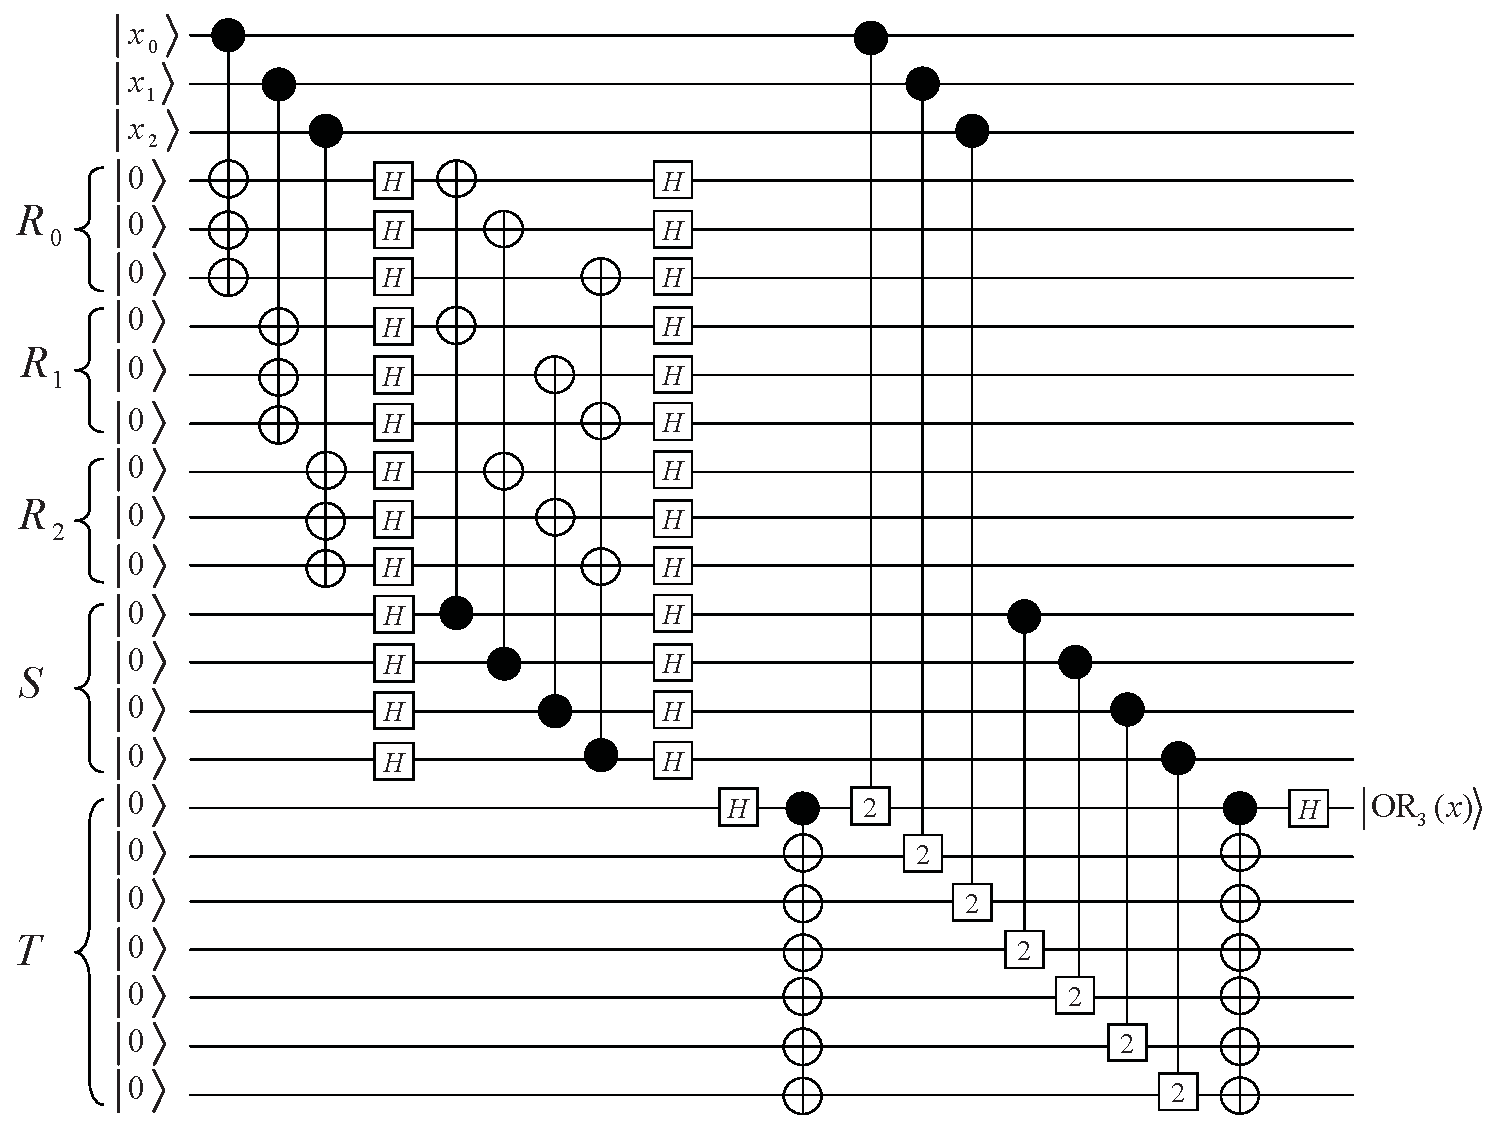
\includegraphics[width=3in]{figures/or3.pdf}
\caption{The constant-depth exact \textsc{OR} circuit on 3 qubits \cite{Takahashi2011}.}
\label{fig:or3}
\end{center}
\end{figure}

While the improvement of $O(\log^*{n})$ depth in the approximate \textsc{OR} case to
$O(1)$ depth in the exact \textsc{OR} case seems like a very small improvement,
the analysis of boolean functions and their decomposition into the
basis of parity functions is a very general technique which could lead to
low-depth circuits in the future, and possibly the discovery of another gate
that is as similarly powerful as unbounded fan-out.